% % !TeX program = xelatex
% !TeX spellcheck = es_ES
% !TeX encoding = utf8

\documentclass[onecolumn,10pt,titlepage,a4paper]{article}

\usepackage[a4paper,top=2.5cm,bottom=2cm,left=2cm,right=2cm,marginparwidth=1.75cm,headheight=28pt]{geometry}
% Formateo para castellano
%\usepackage[utf8]{inputenc}
\usepackage[spanish,mexico]{babel}
%\usepackage{natbib}



%Bibliografía

% Simbolos para notas de pie
\usepackage[symbol]{footmisc}
\renewcommand*{\thefootnote}{\fnsymbol{footnote}}

% \renewcommand{\thefootnote}{\fnsymbol{footnote}}
% \footnote[num]{text}

% \pagestyle{myheading}
% \markright{Mi Documento \hfill Mi nombre \hfi}
%
\usepackage{fancyhdr,framed}
\setlength{\headheight}{15.2pt}
\pagestyle{fancy}
\lhead{Elementos Finitos II - 31.92 \\ Patricio Whittingslow -- 55423}
\chead{TP 2}


%\usepackage{subcaption}

% Para el entorno align


% Multiples columnas para glosario
\usepackage{multicol}

%Figuras y subtitulos
\usepackage{graphicx}
\usepackage{caption,subcaption}
\usepackage{hyperref}
\hypersetup{
    colorlinks,
    citecolor=black,
    filecolor=black,
    linkcolor=black,
    urlcolor=black
}
\usepackage[utopia,expert]{mathdesign} %Opcion "expert" para no romperme las smallcaps de helvetica. 
\usepackage{amsmath}

\newcommand{\rmfont}[1]{{\fontfamily{ptm}\selectfont%
		#1}}
\newcommand{\rmfontbf}[1]{{\fontfamily{ptm}\selectfont%
		\textbf{#1}}}
\newcommand{\rmfontsc}[1]{{\fontfamily{ptm}\selectfont%
		\textsc{#1}}}
    
\newcommand{\Matlab}{\rmfont{\sc Matlab}}
    \newcommand{\Adina}{{\sc ADINA}}
    \newcommand{\refp}[1]{(\ref{#1})}
    \newcommand{\unspace}{\!\!\!\!\!\!\!\!\!\!\!\!\!\!\!\!\!\!\!\!}
    \newcommand{\ms}{\ \ \ } %Matrix Spacing
    \newcommand{\di}{\textrm{d}}
    \newcommand{\jac}{\rmfontbf{J}}
    \newcommand{\Djac}{|\;\jac\;|}
    \newcommand{\dNi}{\di N_i}
    \newcommand{\sigmab}{\boldsymbol{\sigma}}
    \newcommand{\varepsilonb}{\boldsymbol{\varepsilon}}
    \newcommand{\Phib}{\boldsymbol{\Phi}}
    \newcommand{\CPhi}{\boldsymbol{\{ } \Phi \boldsymbol{\} }}
    \newcommand{\Mme}[1]{\boldsymbol{[}\mathbf{#1} \boldsymbol{]}}
    \newcommand{\Rme}[1]{\boldsymbol{\lfloor}\mathbf{#1} \boldsymbol{\rfloor}}
    \newcommand{\Cme}[1]{\boldsymbol{\{ }\mathbf{#1} \boldsymbol{\}} }
    \newcommand{\MB}{\Mme{B}}
    \newcommand{\MN}{\Mme{N}}
    \newcommand{\ME}{\Mme{E}}
    \newcommand{\Mk}{\Mme{k}}
    \newcommand{\MA}{\Mme{A}}
    \newcommand{\radial}{r}
    \newcommand{\eff}{f}
%Helvetica
\renewcommand{\familydefault}{\sfdefault}
\usepackage[scaled=1]{helvet}
\usepackage[format=plain,
            labelfont={bf,it},
            textfont=it]{caption}
%\usepackage[T1]{fontenc}
%--------------------------------------


\usepackage{siunitx}
\newcommand{\glossentry}[2]{$#1\ $ \indent #2 \par \vspace{.4cm} }
\newcommand{\adm}{\textrm{adm}}


\title{Informe Técnico - ITBA}

\author{Patricio Whittingslow}
%========================> Comienza Documento
\begin{document}
\begin{titlepage}
	\centering
	
	{ \large Instituto Tecnológico de Buenos Aires  \par }
	\vspace{2cm}
	{\Large \scshape Elementos Finitos II - 31.92 \par}
	\vspace{2cm}
	{\Huge \scshape Estudio de una viga\par }
	\vspace{.5cm}
	{\Large Y un motor a venir \par}
	\vspace{2cm}
	{\large \bf Autor \par}
	\vspace{.5cm}
	\textsc{\large Patricio Whittingslow -- 55423}
	\vspace{2cm}
	{\par \large Fecha de realización: \today \par}
	\vspace{1cm}
	{\large Fecha de entrega: .......................................\par}
	\vspace{2.5cm}
	{\large Firma del docente: .......................................}
	\vspace{3cm}
	\begin{figure}[htb!]
		\centering
		
\includegraphics[width=6cm]{fig/logoitba.png}
	\end{figure}
\end{titlepage}




\begin{multicols}{2}
	\section*{Glosario}
	\glossentry{\Cme{R}}{Vector de cargas externas.}
	\glossentry{\Mme{K}}{Matriz de rigidez.}
	\glossentry{\Mme{M}}{Matriz de masa.}
	\glossentry{\Cme{D}}{Vector de desplazamientos.}
	\glossentry{p}{Carga de presión.}
	\glossentry{\kappa_{0}}{Curvatura de placa inicial.}
\end{multicols}


\tableofcontents

\section{Introducción Teórica}
Cuando se tiene una carga dependiente del tiempo la respuesta estructural también lo es. En el caso que sea un problema cuasiestático la resolución se puede hacer para los instantes de tiempos interesantes. Caso contrario se precisa efectuar un \textit{análisis dinámico}.
\[
\text{Cuasiestático:}\quad \Mme{K}\Cme{D} = \Cme{R} \longrightarrow \text{Dinámico:} \quad 
\Mme{M} \Cme{\ddot{D}} + \Mme{C}\Cme{\dot{D}} + \Mme{K}\Cme{D} = \Cme{R}	
\]
donde el termino $\Mme{K}\Cme{D}$ suele ser referido como las \textit{fuerzas internas}, y $\Cme{R}$ siendo las \textit{fuerzas externas}.

El análisis dinámico busca la forma de deformación del sistema cuando este se encuentra excitado por cargas a una frecuencia cercana a la natural. La respuesta en deformación del sistema con una carga cíclica puede ser menor o mayor que con cargas estáticas de misma magnitud máxima, pero cuando la frecuencia de carga se acerca a la natural las deformaciones serán mucho mayor. 

Debido a este último punto es de sumo interés conocer la frecuencia natural de un sistema que tiene la posibilidad de someterse a una carga cíclica. Incluso puede ser de gran utilidad conocer el modo de deformación para entender como el sistema almacena energía. Un caso famoso de falla por resonancia es el de \textit{Tacoma Narrows} (Angostas de Tacoma, en español). La sección del puente tenía una forma doble-T acostado que, al girar en presencia de un viento con velocidad particular, creaba una diferencia de presiones excitadora entre el lado superior e inferior así contribuyendo al giro hasta por fin fallar.

{\textbf{Problema}}\par
Hallar para el problema descrito en la figura \ref{fig:enunciado}:
\begin{itemize}
	\item Frecuencias Naturales
	\item Amortiguamiento modal y proporcional
	\item Carga armónica
	\item \textit{Frecuencia de Barrido}
\end{itemize}

\begin{figure}[htb!]
	\centering
	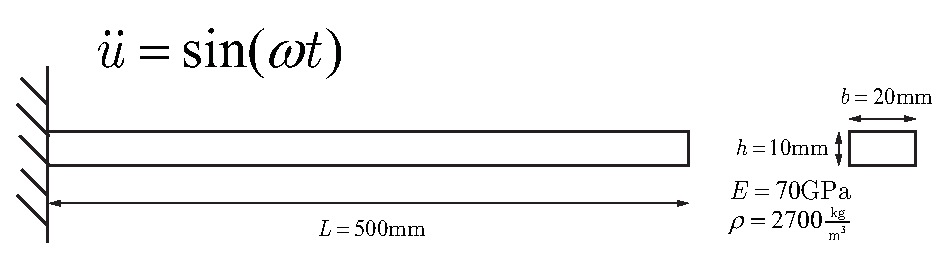
\includegraphics[width=0.6\textwidth]{fig/enunciado.eps}
	\caption{Se resolvió para una viga de aluminio empotrada excitada por una aceleración uniforme.}\label{fig:enunciado}
\end{figure}
Cabe destacar que el enunciado original otorgado por la cátedra sugería usar para la aceleración excitadora $\ddot{u}=\sin (\Omega x)$, el cual nos daría un sistema cuasiestático poco interesante.\footnote{a no ser que $\Omega$ esté en función del tiempo y no se haya especificado}

\section{Método}
Se resuelve el problema por método de los elementos finitos utilizando vigas de dos nodos. Cada nodo tiene dos grados de libertad, $v$ como el desplazamiento en $y$ y $\theta$ siendo el giro de la viga en el plano $x\!y$.

La matriz de masa usada es \textit{consistente}. Esta y la matriz de rigidez toman la forma: \cite[p.379]{cook2007concepts}
\[
\Mme{m}_{\mathrm{viga}}=\frac{\rho A L}{420}\left[\begin{array}{cccc} 156 & 22\,\mathrm{L} & 54 & -13\,\mathrm{L}\\ 22\,\mathrm{L} & 4\,{\mathrm{L}}^2 & 13\,\mathrm{L} & -3\,{\mathrm{L}}^2\\ 54 & 13\,\mathrm{L} & 156 & -22\,\mathrm{L}\\ -13\,\mathrm{L} & -3\,{\mathrm{L}}^2 & -22\,\mathrm{L} & 4\,{\mathrm{L}}^2 \end{array}\right] \qquad \qquad \Mme{k}_{\mathrm{viga}}=\frac{E I_z}{L^3} \left[\begin{array}{cccc} 12 & 6\,L & -12 & 6\,L\\ 6\,L & 4\,L^2 & -6\,L & 2\,L^2\\ -12 & -6\,L & 12 & -6\,L\\ 6\,L & 2\,L^2 & -6\,L & 4\,L^2 \end{array}\right]
\]

Se resuelve el problema de autovalores para el sistema sin amortiguamiento \eqref{eq:eigenvalueproblem} y se obtienen las frecuencias naturales del sistema 

\begin{equation} \label{eq:eigenvalueproblem}
	\left( \Mme{K} - \omega^2 \Mme{M}\right)\Cme{D}= 0
\end{equation}

Luego se busca la respuesta armónica del sistema ante la carga conocida. La formulación \textbf{modal} es la siguiente
\begin{equation} \label{eq:Zmodal}
	\Cme{Z} = \frac{\Cme{R\modal }}{{\Cme{\Omega}}^2 \sqrt{(1-\chi^2)^2 + (2 \dampfact \chi)^2}}
\end{equation}
donde $\chi = \frac{\omega_{\mathrm{exc}}}{\Cme{\Omega}}$ y $\dampfact$ se elige a criterio del usuario.

La formulación \textbf{proporcional} propone que el amortiguamiento es una combinación lineal de la masa y la rigidez. Se propone estudiar la respuesta proporcional de la misma forma que la modal según:
\begin{equation}
	\Cme{D} = \frac{\Cme{R }}{{\Cme{\Omega}}^2 \sqrt{(1-\chi^2)^2 + (2 \dampfact \chi)^2}}
\end{equation}
donde $\chi = \frac{\omega_{\mathrm{exc}}}{\Cme{\Omega}}$ y 
$\dampfact = \tfrac{1}{2} \left(\frac{\alpha}{\omega_{\mathrm{exc}}} +\beta \omega_{\mathrm{exc}} \right) $.
Si se quiere estudiar un rango de frecuencias excitadoras tal que $\omega_{\mathrm{exc}}\in [\omega_1, \omega_2]$ y eligiendo dos valores de amortiguamiento para ambas frecuencias $\dampfact_1$ y $\dampfact_2$ se tiene: \cite{cook2007concepts}
\begin{align} \label{eq:alfabeta}
\alpha &= 2\omega_1 \omega_2 (\dampfact_1 \omega_2 -\dampfact_2 \omega_1)/(\omega_2^2 - \omega_1^2) \\ \beta &= 2(\dampfact_2\omega_2 -\dampfact_1 \omega_1)/(\omega_2^2 - \omega_1^2)
\end{align}

Se opta por estudiar el rango de amortiguamiento  $\varsigma\in \{0,05;\, 0,3\}$. Este es el rango inferior por donde se puede encontrar el amortiguamiento para problemas similares al enunciado.
\begin{itemize}
	\item Para el barrido de frecuencias de amortiguamiento proporcional se investigará el caso donde se elija $\varsigma_1=0,05$ fijo y variando $\varsigma_2$ para obtener las curvas de respuesta a frecuencia.
	\item El otro caso investigado será $\varsigma_2=0,3$ fijo variando así $\varsigma_1$.
\end{itemize}

\section{Resultados}
Las primeras tres frecuencias naturales obtenidas con una solución de 8 elementos.
\[
\Cme{\Omega} = \begin{Bmatrix}
\vdots \\
7259 \si{\, \radian \per \second}\\
2591 \si{\, \radian \per \second}\\
413 \si{\, \radian \per \second}
\end{Bmatrix}=\begin{Bmatrix}
\vdots \\
1155\, \textrm{hz}\\
412\, \textrm{hz}\\
65,8\, \textrm{hz} 
\end{Bmatrix}
\]

\begin{figure}[htb!] 
	\centering
	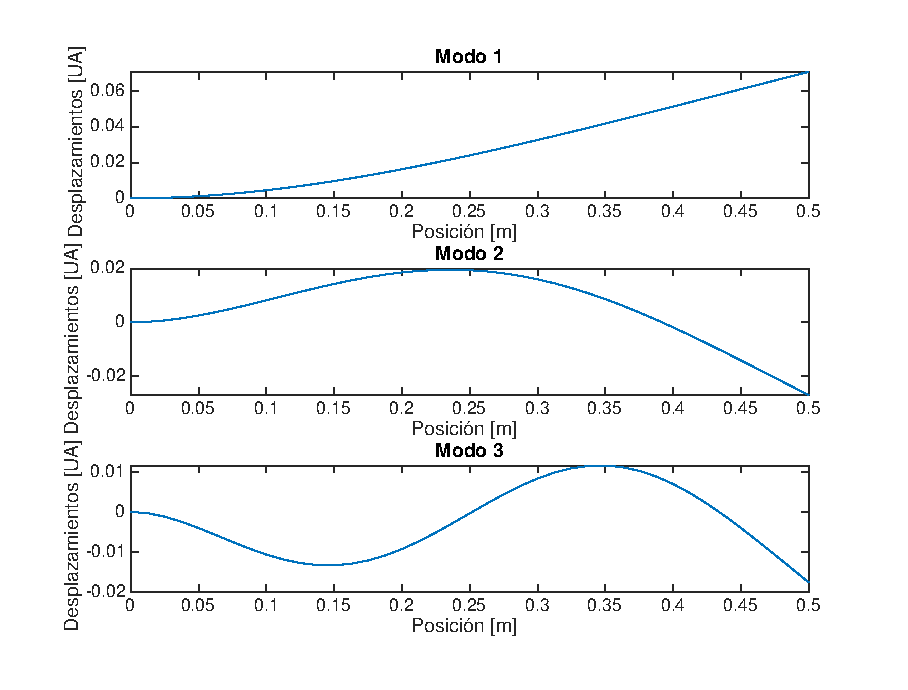
\includegraphics[width=1\textwidth]{fig/modos.eps}
	\caption{Modos de deformación para las frecuencias naturales. El modo 1 corresponde a la frecuencia más baja.}
	\label{fig:modos}
\end{figure}

\begin{figure}[htb!]
	\centering
	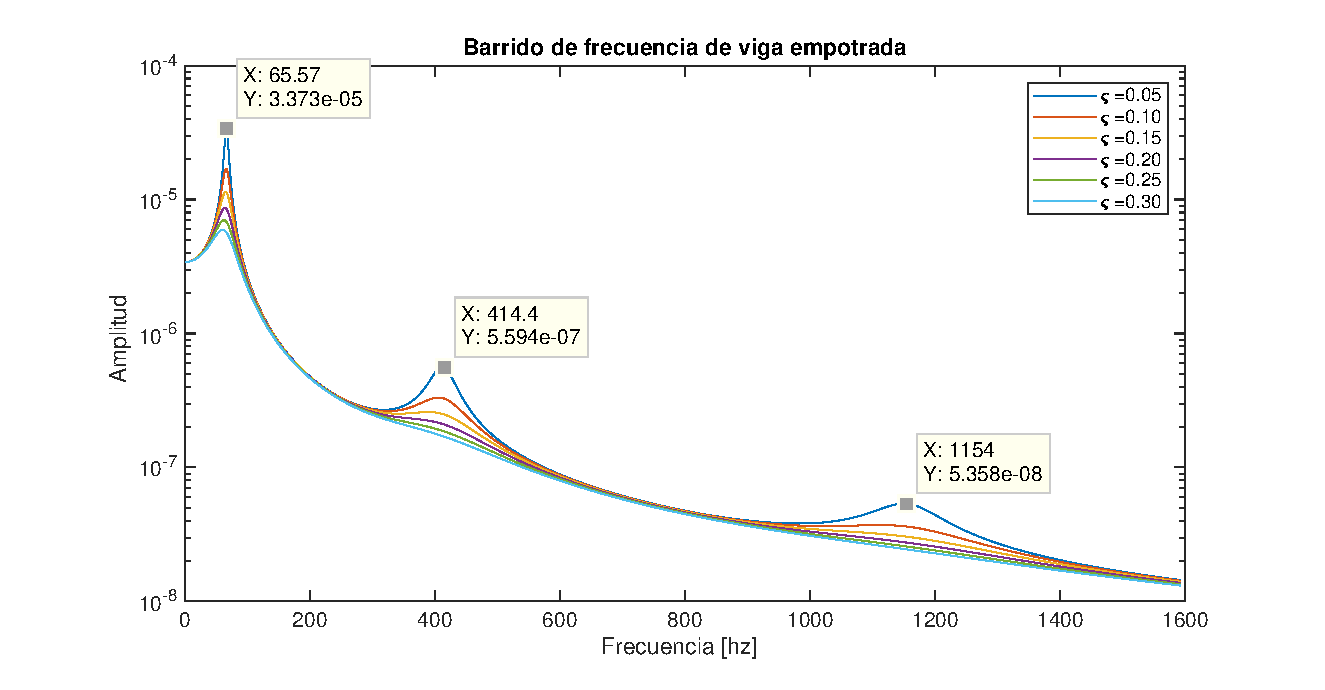
\includegraphics[width=1\textwidth]{fig/sinesweep.eps}
	\caption{Barrido de frecuencia \textbf{modal}. Valores de amplitud máxima recuadrados.}
	\label{fig:sinesweepmodal}
\end{figure}

\begin{figure}[htb!]
	\centering
	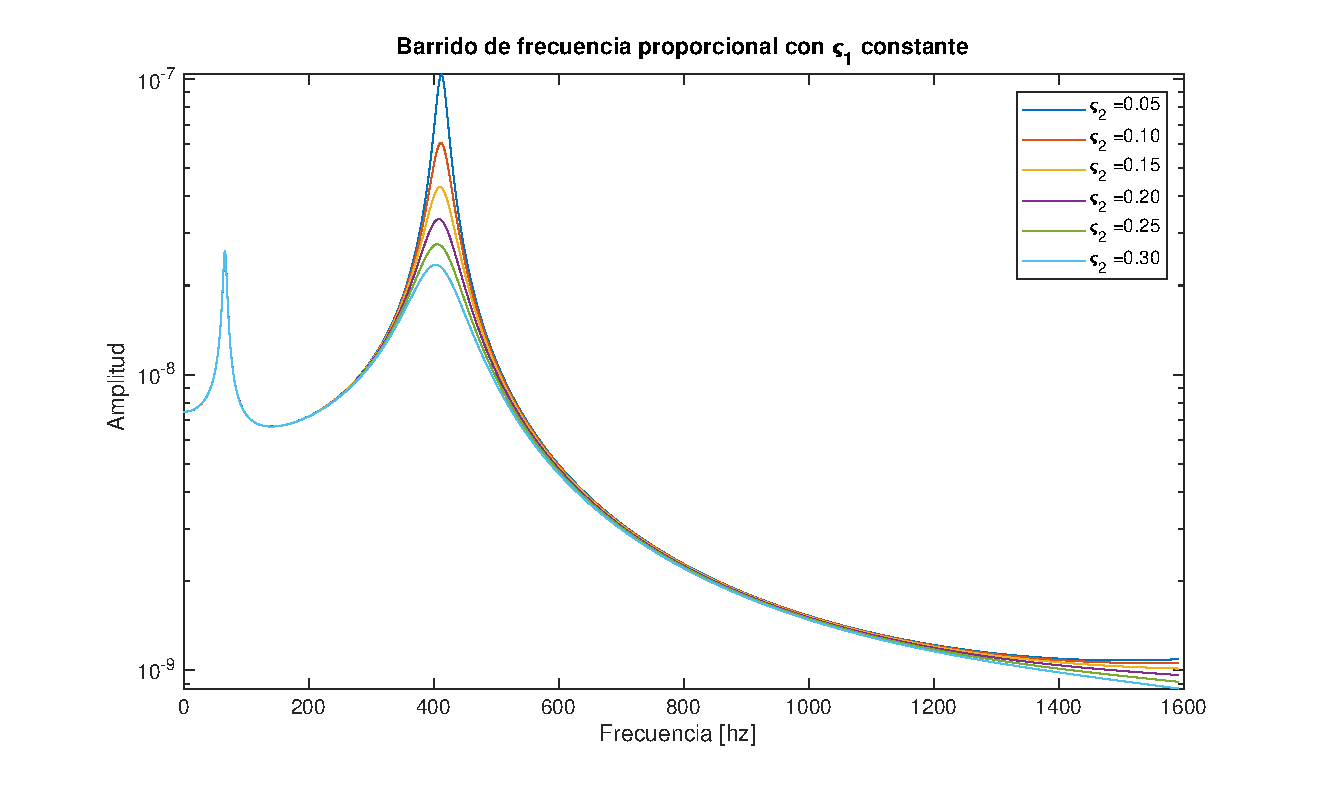
\includegraphics[width=1\textwidth]{fig/sinesweepprop1const.eps}
	\caption{Barrido de frecuencia \textbf{proporcional}.}
	\label{fig:sinesweepprop1}
\end{figure}

\begin{figure}[htb!]
	\centering
	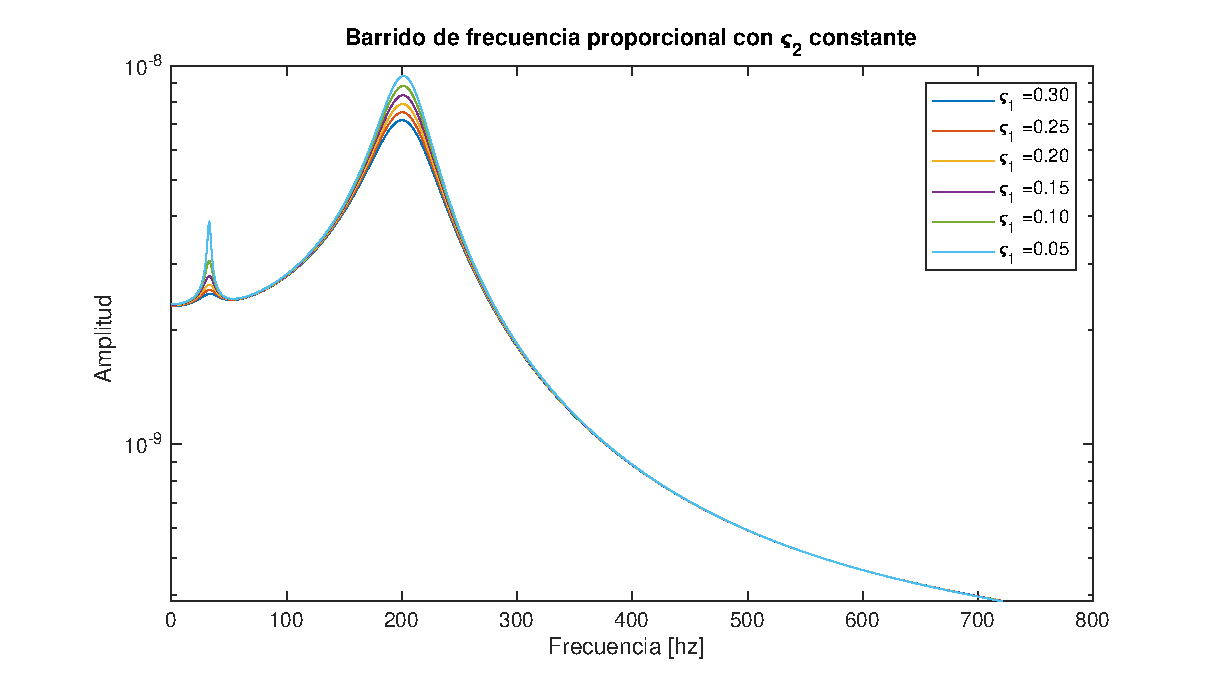
\includegraphics[width=1\textwidth]{fig/sinesweepprop2const.eps}
	\caption{Barrido de frecuencia \textbf{proporcional}.}
	\label{fig:sinesweepprop2}
\end{figure}





\clearpage
\section{Conclusiones}
Se informa al lector el hallazgo de la frecuencias naturales. Dichas frecuencias están separadas por un $\Delta \omega $ considerable. Esto es deseable para cuando se tenga una carga cíclica esta trabaje lejos de cualquier frecuencia natural, y si es posible, por debajo de todas. Dado que no se especifico ninguna característica técnica del problema, el gráfico \ref{fig:modos} es más una curiosidad. Las formas de los modos no están a escala ni tienen unidades, es solo la forma de respuesta. 

A medida que la frecuencia de excitación aumenta la \textit{amplitud del sistema disminuye}\footnote{Excepto en cercanías de una frecuencia natural} (ver figura \ref{fig:sinesweepmodal}). Es interesante pensar que si aumentara no tendría sentido buscar las frecuencias naturales porque estas son caracterizadas por un máximo de amplitud. Las curvas del barrido de frecuencia son decrecientes en lejanía de una frecuencia natural porque para una fuerza cíclica $F(t)=F_0\sin \omega t$ el tiempo que actúa en una dirección es inversamente proporcional a la frecuencia. Por ende la estructura no tiene tiempo para moverse lejos antes de que se invierta la dirección de la fuerza.

El efecto del amortiguamiento es reducir la amplitud cerca de la frecuencia natural. En la figura \ref{fig:sinesweepmodal} se puede apreciar el efecto claramente. Las siguientes dos figuras (\ref{fig:sinesweepprop1} y \ref{fig:sinesweepprop2}) tienen un nivel agregado de profundidad. Se estudia el efecto la \textit{fracción de amortiguamiento crítico} \cite{cook2007concepts} cuando se varían los amortiguamientos de los puntos borde del espectro de diseño. Como es de esperar para un valor mayor $\dampfact_1$ se amortiguarán las frecuencias más bajas sin efecto a frecuencias altas. De forma complementaria, si se aumenta $\dampfact_2$ la amplitud de la primera frecuencia natural no se ve afectada mientras que a frecuencias más altas se reduce la amplitud considerablemente.


\bibliography{labibliografia} % Indica archivo
\bibliographystyle{plainnat} 

\end{document}